\documentclass{article}
% Text
\usepackage[utf8]{inputenc}
\usepackage[spanish]{babel}
\usepackage{enumitem}
% Images
\usepackage{graphicx}
\graphicspath{ {./images/} }
% Math
\usepackage{amsmath}
\usepackage{amsthm}
\usepackage{amsfonts}
\usepackage{amssymb}
\usepackage{physics}
\usepackage{bbm}
% Math symbols
\DeclareMathOperator{\prob}{\mathbb{P}}
\DeclareMathOperator{\Exp}{\mathbb{E}}
\DeclareMathOperator{\Exponential}{\text{Exp}}
\DeclareMathOperator*{\argmin}{\text{argmín}}
\newcommand{\symmetric}{\mathbb{S}}
\newcommand{\naturalnum}{\mathbb{N}}
\newcommand{\realnum}{\mathbb{R}}
\newcommand{\characteristic}{\mathbbm{1}}
% Math environments
\newtheorem{theorem}{Teorema}
\theoremstyle{definition}
\newtheorem{definition}{Definición}
\newtheorem{exercise}{Ejercicio}

\title{Ejercicios para entregar}
\author{Pablo Brianese}

\begin{document}
\maketitle

\begin{exercise}
Consideremos un sistema que tiene un único servidor, que atiende a tasa $\mu > 0$, y los clientes llegan a tasa $\lambda > 0$.
Sea $X_t$ la cantidad de clientes que hay en la cola a tiempo $t$, con $t \geq 0$.
Notar que $(X_t)_{t \geq 0}$ es un proceso de Markov a tiempo continuo.
(Este modelo, llamado $M/ M / 1$, lo hemos charlado en la clase práctica 20 y 23).
\begin{enumerate}[label=\alph*)]
    \item Probar que el proceso es recurrente positivo si y sólo si $\lambda < \mu$.
	Con lo cual, empezando con la cola vacía, el tiempo medio que tarda la cola en volver a vaciarse es finito si y sólo si $\lambda < \mu$.
	\item Asumiendo $\lambda < \mu$, calcular la proporción (asintótica) de tiempo que la cola está vacía.
\end{enumerate}
\end{exercise}

\begin{proof} a)
Elaboramos el punto según el cual \((X_t)_{t \geq 0}\) es un proceso de Markov a tiempo continuo con espacio de estados numerable \(I =  \naturalnum_0 = \{0, 1, 2, \dots\}\).

Si el proceso está en el estado 0 (no hay clientes en la cola), sólo puede saltar al estado 1 (llega un nuevo cliente). 
Y esto sucede cuando suena un reloj exponencial de parámetro \(\lambda\).
Por el contrario, si su estado es \(i > 0\) (hay \(i\) clientes esperando a ser atendidos), puede saltar a \(i - 1\) (un cliente es atendido y se retira) o a \(i + 1\) (un nuevo cliente se suma a la cola).
Y esta transición obedece a la competencia de dos relojes exponenciales, uno a tasa \(\lambda\) (que indica la llegada de una persona), y otro a tasa \(\mu\) (que indica que una se va).
Por lo tanto, la matriz \(Q = (q_{i j})_{i, j \in I}\) de tasas de transición de la cadena está dada por
\begin{align}
	Q
	&=
	\begin{pmatrix}
		- \lambda &\lambda \\
		\mu &- (\lambda + \mu) &\lambda \\
		 &\mu &- (\lambda + \mu) &\lambda \\
		 & &\mu &- (\lambda + \mu) &\lambda \\
		 & & &\ddots &\ddots &\ddots
	\end{pmatrix}
\end{align}
Es decir:
\begin{align}
	q_{0 0} &= - \lambda & &q_{0 1} = \lambda,
	\\
	q_{i i} &= - (\lambda + \mu) & &\begin{aligned}q_{i, i-1} &= \mu,\\ q_{i, i+1} &= \lambda \end{aligned} &&(\forall i > 0)
\end{align}
siendo nulas las entradas que no figuran en esta descripción.

% teorica22.pdf <-- por acá empieza la relación entre las matrices Q y Pi.

% Para probar este teorema es clave el teorema de teorica24.pdf Pág. 1 sobre recurrencia positiva y matrices generadoras irreducibles.

Sea \(T_i = \inf\{t > J_1 : X_t = i\}\) para cada \(i \in I\).
Un estado \(i \in I\) será recurrente si \(\prob^i(T_i<\infty)=1\).
Será recurrente positivo si \(\Exp^i(T_i) < \infty\).

% teorica23.pdf %
%%%%%%%%%%%%%%%%%
\begin{definition}
Decimos que una matriz generadora \(Q\) es irreducible si para todo par de estados \(i, j \in I\) existe un camino \(i_0, i_1, \dots, i_k\) entre ellos (\(i_0 = i\), \(i_k = j\)) tal que las tasas \(q_{i_0 i_1}, q_{i_1 i_2}, \dots, q_{i_{k - 1} i_k}\) son positivas.
\end{definition}

% El proceso de Markov es irreducible %
%%%%%%%%%%%%%%%%%%%%%%%%%%%%%%%%%%%%%%%
En virtud de las tasas de transición \(q_{01} = \lambda\), \(q_{i, i + 1} = \mu\), \(q_{i, i + 1} = \lambda\) con \(\mu, \lambda > 0\), se sigue que la matriz generadora \(Q\) de nuestro modelo M/M/1 es irreducible.

% teorica24.pdf %
%%%%%%%%%%%%%%%%%
\begin{theorem} % Tengo que cambiar esta \nu por otro símbolo
Sea \((X_t)_{t \geq 0}\) un proceso de Markov en un espacio de estados \(I\) numerable, con tasas \((\lambda(i))_{i \in I}\) y matriz generadora \(Q\) irreducible.
Son equivalentes:
\begin{enumerate}
	\item todo estado es recurrente positivo;
	\item existe un estado \(i \in I\) recurrente positivo;
	\item \(Q\) tiene una distribución \(\nu\) tal que \(\nu^{T} Q = 0\).
\end{enumerate}
En cualquiera de los casos la distribución invariante \(\nu\) es igual a
\begin{align}
	\nu(i) = \frac{1}{\lambda(i) m_i}
\end{align}
donde \(m_i = \Exp^i(T_i)\).

% La matriz generadora es irreducible %
%%%%%%%%%%%%%%%%%%%%%%%%%%%%%%%%%%%%%%%
\begin{proof}
Sea \(\nu = (\nu_i)_{i \in I}\) un vector.

Supongamos que \(\nu^T Q = 0\), es decir que contamos con la ecuación \(\sum_{i \in I} \nu_i q_{i j} = 0\) para todo \(j \in I\).
Analizando esta ecuación en el caso \(j = 0\) vemos que \(\nu_0 (- \lambda) + \nu_1 \mu = 0\), y en particular \(\nu_1 = (\lambda / \mu) \nu_0\).
Digamos que \(\rho = \lambda / \mu\), de modo tal que 
\begin{align}
	\nu_1 = \rho \nu_0
\end{align}
Para \(j = 1\) tenemos \(\nu_0 \lambda + \nu_1 (- (\lambda + \mu)) + \nu_2 \mu = 0\).
Dividiendo por \(\mu > 0\), se sigue \(\nu_0 \rho + \nu_2 = \nu_1 (\rho + 1)\).
Además, usando \(\nu_1 = \rho \nu_0\), obtenemos \(\nu_1 + \nu_2 = \nu_1 (\rho + 1)\).
Luego 
\begin{align}
	\nu_2 = \rho \nu_1
\end{align}
Supongamos, a fin de concretar un argumento inductivo, que esta relación \(\nu_{j + 1} = \rho \nu_j\) se sostiene para \(j \in \{0, 1, \dots, k\}\) con \(k \geq 1\).
Entonces la ecuación \(\sum_{i \in I} \nu_i q_{i, k} = 0\) dice \(\nu_{k - 1} \lambda + \nu_k (- (\lambda + \mu)) + \nu_{k + 1} \mu = 0\), porque \(k \geq 1\).
Dividiendo por \(\mu > 0\), se sigue \(\nu_{k - 1} \rho + \nu_{k + 1} = \nu_k (\rho + 1)\).
Usando nuestra hipótesis inductiva para \(k - 1 \leq k\) obtenemos la ecuación \(\nu_k = \rho \nu_{k - 1}\), y con esta deducimos \(\nu_k + \nu_{k + 1} = \nu_k (\rho + 1)\).
Luego
\begin{align}
	\nu_{k + 1} = \rho \nu_k
\end{align}
Lo cual lleva el conjunto de valores \(j \in I\) que verifican la relación \(\nu_{j + 1} = \rho \nu_j\) a \(\{0, 1, \dots, k, k + 1\}\).
Por inducción, \(\nu_{j + 1} = \rho \nu_j\) para todo \(j \in I\).
De esta relación de recurrencia se sigue la identidad 
\begin{align}
	&\nu_i = \rho^i \nu_0 &&(\forall i \in I)
\end{align}

% Acá tengo que poner la ecuación nu = rho^i nu0
% De esa ecuación se deducirá la doble equivalencia con mu > lambda.
Recíprocamente, supongamos que \(\nu = (\rho^i \nu_0)_{i \in I}\) y probemos \(\nu^T Q = 0\).
Tenemos que probar \(\sum_{i \in I} \nu_i q_{i j} = 0\) para todo \(j \in I\).
En el caso \(j = 0\) tenemos que probar \(\nu_0 (- \lambda) + (\rho \nu_0) \mu = 0\), y esta ecuación se sigue fácilmente de la definición \(\rho = \lambda / \mu\).
En el caso \(j \geq 1\) tenemos que probar \((\rho^{j - 1} \nu_0) \lambda + (\rho^j \nu_0) (- (\lambda + \mu)) + (\rho^{j + 1} \nu_0) \mu = 0\).
Dividiendo por \(\mu\) esto se transforma en \(\rho^j \nu_0 + \rho^{j + 2} \nu_0 \mu = \rho^{j + 1} \nu_0 (\rho + 1)\)



Si \(\nu_0 = 0\), entonces \(\nu = 0\) y la ecuación \(\nu^T Q = 0\) resulta trivial.
Consideremos el caso contrario en que \(\nu_0 > 0\).
Aquí corresponde analizar el efecto de \(\rho\).
Si \(\rho = 1\), entonces \(\nu = (\nu_0)_{i \in I}\) es una medida infinita sobre \(I\) --- se verifica \(\sum_{i \in I} \nu_i = \infty\).
Si \(\rho \neq 1\), entonces \(\nu = (\rho^i \nu_0)_{i \in I}\).
En el caso \(\rho > 1\) se tiene \(\lim_{i \rightarrow \infty} \rho^i = \infty\), lo cual hace de \(\nu\) una medida infinita --- se verifica \(\sum_{i \in I} \nu_i = \infty\).
En contraste, cuando \(\rho < 1\)
\end{proof}

\end{theorem}





% Nota 25 nov. 2020 teoría de proba  clase práctica 20.pdf %
%%%%%%%%%%%%%%%%%%%%%%%%%%%%%%%%%%%%%%%%%%%%%%%%%%%%%%%%%%%%
Vamos a ver que \(\Exp(T_0) < \infty\) si y solo si \(\lambda < \mu\).

Si la cadena está en el estado 0, sólo puede saltar al 1; si está en un estado \(i > 0\), puede saltar a \(i - 1\) o a \(i + 1\).

Si está en 0, salta al estado 1 cuando suena un reloj exponencial de parámetro \(\lambda\).
Si se encuntra en un estado \(i > 0\), hay dos relojes exponenciales compitiendo, uno a tasa \(\lambda\), que indica la llegada de una persona y otra a tasa \(\mu\) que indica que una se va. 

Usaremos los siguientes lemas sobre la distribución exponencial:
\begin{enumerate}
	\item Si \(X \sim \Exponential(\lambda)\), entonces \(\prob(X > t + s | X > s) = \prob(X > t)\).
	\item Si \(\{X_i\}_{i \in \naturalnum_0}\) son v.a. independientes con distribuciones \(X_i \sim \Exponential(\lambda_i)\) tales que \(\sum_{i \in \naturalnum_0} \lambda_i\), entonces
	\begin{itemize}
		\item \(\min_{i \in \naturalnum_0} X_i \sim \Exponential(\lambda)\) con \(\lambda = \sum_{i \in \naturalnum_0} \lambda_i\)
		\item \(\prob(\argmin_{i \in \naturalnum_0} X_i = j) = \lambda_j / \lambda\), con \(\lambda = \sum_{i \in \naturalnum_0} \lambda_i\), para todo \(j \in \naturalnum_0\).
	\end{itemize}
\end{enumerate}

Usando estos lemas, podemos pensar que estando la cadena en el estado \(i > 0\), su cambio responde a un único reloj exponencial con tasa \(\lambda + \mu\), y al sonar este reloj se tira una moneda cargada:
con probabilidad \(\lambda / (\lambda + \mu)\) salta al estado \(i + 1\), y con probabilidad \(\mu / (\lambda + \mu)\) salta al estado \(i - 1\).
%%%%%%%%%%%%%%%%%%%%%%%%%%%%%
\end{proof}

%%%%%%%%%%%%%%%%%%%%%%%%%%%%%%
\begin{exercise}
Consideremos un sistema de $n \in \naturalnum$ servidores, en donde cada servidor atiende a tasa $\mu > 0$, y los clientes arriban al sistema a tasa $\lambda > 0$.
(Los tiempos de duración de los servicios tienen distribución exponencial con parámetro $\mu$, independientes entre sí, e independientes al proceso de llegada de los clientes, que siguen un proceso de Poisson de tasa $\lambda$).

Si un cluente llega y encuentra todos los servidores ocupados, automáticamente se va.
En caso contrario, el cliente ingresa al sistema, ubicándose en algún servidor que estaba desocupado, y luego de ser atendido, se va del sistema.

Llamemos $X_t$ a la cnatidad de servidores ocupados a tiempo $t$, $t \geq 0$.
Observemos que $(X_t)_{t \geq 0}$ es un proceso de Markov a tiempo continuo, donde el espacio de estados es $S = \{0, 1, \dots, n\}$, y el diagrama de las tasas de transición es
\begin{center}
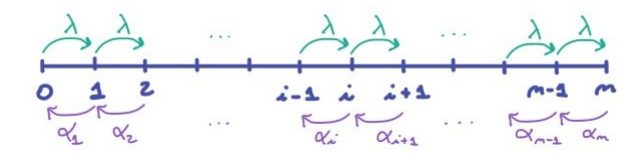
\includegraphics[width=0.75\textwidth]{diagrama_de_las_tasas_de_transicion}
\end{center}
para ciertos valores $\alpha_1, \alpha_2, \dots, \alpha_n$.
\begin{enumerate}[label=\roman*.]
	\item Hallar la probabilidad de que el primer cliente en arribar al sistema encuentre exactamente $k$ servidores ocupados (es decir, que al instante en el que arriba el primer cliente, el proceso $(X_t)_{t \geq 0}$ pase de $k$ a $k + 1$).
	\item Hallar la probabilidad de que el primer cliente en arribar al sistema encuentre exactamente $i$ servidores ocupados, con $i \in S$.
(Pensar primero el caso $i = k - 1$, $i = k - 2$, ect.)
	\item Hallar el número esperado de servidores ocupados que encuentra el primer cliente que arriba al sistema.
\end{enumerate}
\end{exercise}

%%%%%%%%%%%%%%%%%%%%%%%%%%%%%%
\begin{exercise}
Sea $(B_t)_{t \geq 0}$ un Movimiento Browniano estándar en dimensión 1.

Para cada $x \in \realnum$ sea $T_x = \inf \{t \geq 0 : B_t = x\}$.
(Notar que \(T_0 = 0\) a.s.)
Denotamos con \(f_{T_x}\) y \(F_{T_x}\) a la función de densidad y a la función de distribución acumuladad de \(T_x\), respectivamente.
\begin{enumerate}[label=\alph*)]
	\item Probar que \(\prob(T_x < + \infty) = 1\) para todo \(x \in \realnum\).
	(Sugerencia: puede ser útil observar el \(\sup_{t \geq 0} B_t\) y el \(\inf_{t \geq 0} B_t\))
	\item Para cada \(x \in \realnum \setminus \{0\}\), calcular \(f_{T_x}\) y verificar que \(\Exp(T_x) = + \infty\).
\end{enumerate}
\end{exercise}

%%%%%%%%%%%%%%%%%%%%%%%%%%%%%%
\begin{exercise}
Sea \((B_t)_{t \geq 0}\) un Movimiento Browniano estándar en dimensión 1, y sean \(x > 0\), \(y > 0\).
Consideremos el stopping time \(T = T_{- y} \wedge T_x\).
\begin{itemize}
	\item Probar que \((B_t^2 - t)_{t \geq 0}\) es una martingala.
	\item Probar que \(\Exp(T) = xy\)
\end{itemize}
\end{exercise}

%%%%%%%%%%%%%%%%%%%%%%%%%%%%%%
\begin{exercise}
(Este ejercicio no es obligatorio)

Sea \((B_t)_{t \geq 0}\) un Movimiento Browniano estándar en dimensión 1, y sean \(a > 0\), y \(b > 0\).
El objetivo es probar que \(\prob(B_t = a + b t \text{ para algún } t > 0) = e^{- 2 a b}\).
\begin{enumerate}[label=\alph*)]
	\item Sea \((X_t)_{t \geq 0}\) el proceso definido por \(X_t = e^{2 b B_t - 2 b^2 t}\).
	Probar que \((X_t)_{t \geq 0}\) es una martingala.
	\item Consideremos el stopping time \(T = \inf \{t > 0 : B_t = a + b t\}\) (donde \(T\) lo definimos como \(\infty\) si ese conjunto es vacío, es decir, si \(B_t < a + b t\) para todo \(t > 0\)).
	Probar que \(\Exp(X_T) \characteristic_{T < \infty} = 1\).
	\item Probar que \(\Exp(X_T \characteristic_{T < \infty}) = e^{2 a b} \prob(T < \infty)\).
	\item Concluir que \(\prob(B_t = a + b t\text{ para algún } t > 0) = e^{- 2 a b}\).
\end{enumerate}
\end{exercise}

\end{document}
